\input{\string~/Documents/Latex/header.tex}
\fancyhead[L]{ \myfont August 1st 2019}
\fancyhead[C]{ \myfont CME 253A}
\fancyhead[R]{ \myfont Paul Summers}
\begin{document}
\myfont %you have to use this to make it work
\section*{\myfont Introduction} % (fold)
The world is complicated. We build models to help understand this. Matrix methods are hard, iterative finite difference methods are slow, but GPU methods speed this up.
% section introduction (end)
\section*{\myfont Motivation} % (fold)

One such example of this is viscous flow. Viscous flow can be modeled in matrix form, but for non-linear or multiphase flows, an iterative forward pseudo-time stepping model can prove to be faster and simpler if successfully parallelized. We do not consider a non-linear viscosity ($\eta$) here, but point out that one easily could.

The test case considered here is one of a negatively buoyant ball in a background of lighter viscous fluid. We calculate the initial state, and do not forward step in time, though we would point out this is also easily possible in our model. 
% section motivation (end)
\section*{\myfont Mathematical Model} % (fold)
\begin{equation}
	\frac{1}{k}\frac{\partial P}{\partial t} = -\left(\frac{\partial v_x}{\partial x} + \frac{\partial v_y}{\partial y} + \frac{\partial v_z}{\partial z}\right)
\end{equation}
\begin{equation}
	\rho \frac{\partial v_x}{\partial t} = - \frac{\partial P}{\partial x} + \frac{\partial \tau_{xx}}{\partial x} + \frac{\partial \tau_{xy}}{\partial y} + \frac{\partial \tau_{xz}}{\partial z}
\end{equation}
\begin{equation}
	\rho \frac{\partial v_y}{\partial t} = - \frac{\partial P}{\partial y} + \frac{\partial \tau_{yy}}{\partial y} + \frac{\partial \tau_{xy}}{\partial x} + \frac{\partial \tau_{yz}}{\partial z}
\end{equation}
\begin{equation}
	\rho \frac{\partial v_z}{\partial t} = - \frac{\partial P}{\partial z} + \frac{\partial \tau_{zz}}{\partial z} + \frac{\partial \tau_{xz}}{\partial x} + \frac{\partial \tau_{yz}}{\partial y}
\end{equation}
\begin{equation}
	\tau_{xx} = 2 \eta \left( \frac{\partial v_x}{\partial x} - \frac{1}{3}\left(\frac{\partial v_x}{\partial x} + \frac{\partial v_y}{\partial y} + \frac{\partial v_z}{\partial z}\right)\right)
\end{equation}
\begin{equation}
	\tau_{yy} = 2 \eta \left( \frac{\partial v_y}{\partial y} - \frac{1}{3}\left(\frac{\partial v_x}{\partial x} + \frac{\partial v_y}{\partial y} + \frac{\partial v_z}{\partial z}\right)\right)
\end{equation}
\begin{equation}
	\tau_{yy} = 2 \eta \left( \frac{\partial v_y}{\partial y} - \frac{1}{3}\left(\frac{\partial v_x}{\partial x} + \frac{\partial v_y}{\partial y} + \frac{\partial v_z}{\partial z}\right)\right)
\end{equation}
\begin{equation}
	\tau_{xy} = \eta \left(\frac{\partial v_x}{\partial y} + \frac{\partial v_y}{\partial x}\right)
\end{equation}
\begin{equation}
	\tau_{xz} = \eta \left(\frac{\partial v_x}{\partial z} + \frac{\partial v_z}{\partial x}\right)
\end{equation}
\begin{equation}
	\tau_{yz} = \eta \left(\frac{\partial v_z}{\partial y} + \frac{\partial v_y}{\partial z}\right)
\end{equation}
% section mathmatical_model (end)
\section*{\myfont Numerical Approach} % (fold)
We use pseudo time stepping to accelerate convergence. We iterate until convergence when the max residual is less than a threshold value ($10^{-6}$ in this study). 
$$A^{[k+1]} = A^{[k]} + \Delta \tau_A g_A^{[k]}$$
$$g_A^{[k]} = f_A^{[k]} + (1+\nu/n_i)g_A^{[k-1]}$$
For our specific case, the only time derivatives, so this only applies to iterations of velocity. $f_A$ is the right hand side of the velocity equations (2-4 above), which are also the residuals as the system is at equilibrium when $f_A=0$. We store 3 values of $g_A$ as well as 3 values of $f_A$ (1 of each for each velocity) for every grid point in our model. While this significantly increases the memory load of each iteration, the speed in convergence makes it still more performant that a non-damps iterative method. 

% section numerical_approach (end)
\section*{\myfont Results} % (fold)
2D Cross section of final solution (255x255x255 run)
\begin{center}
	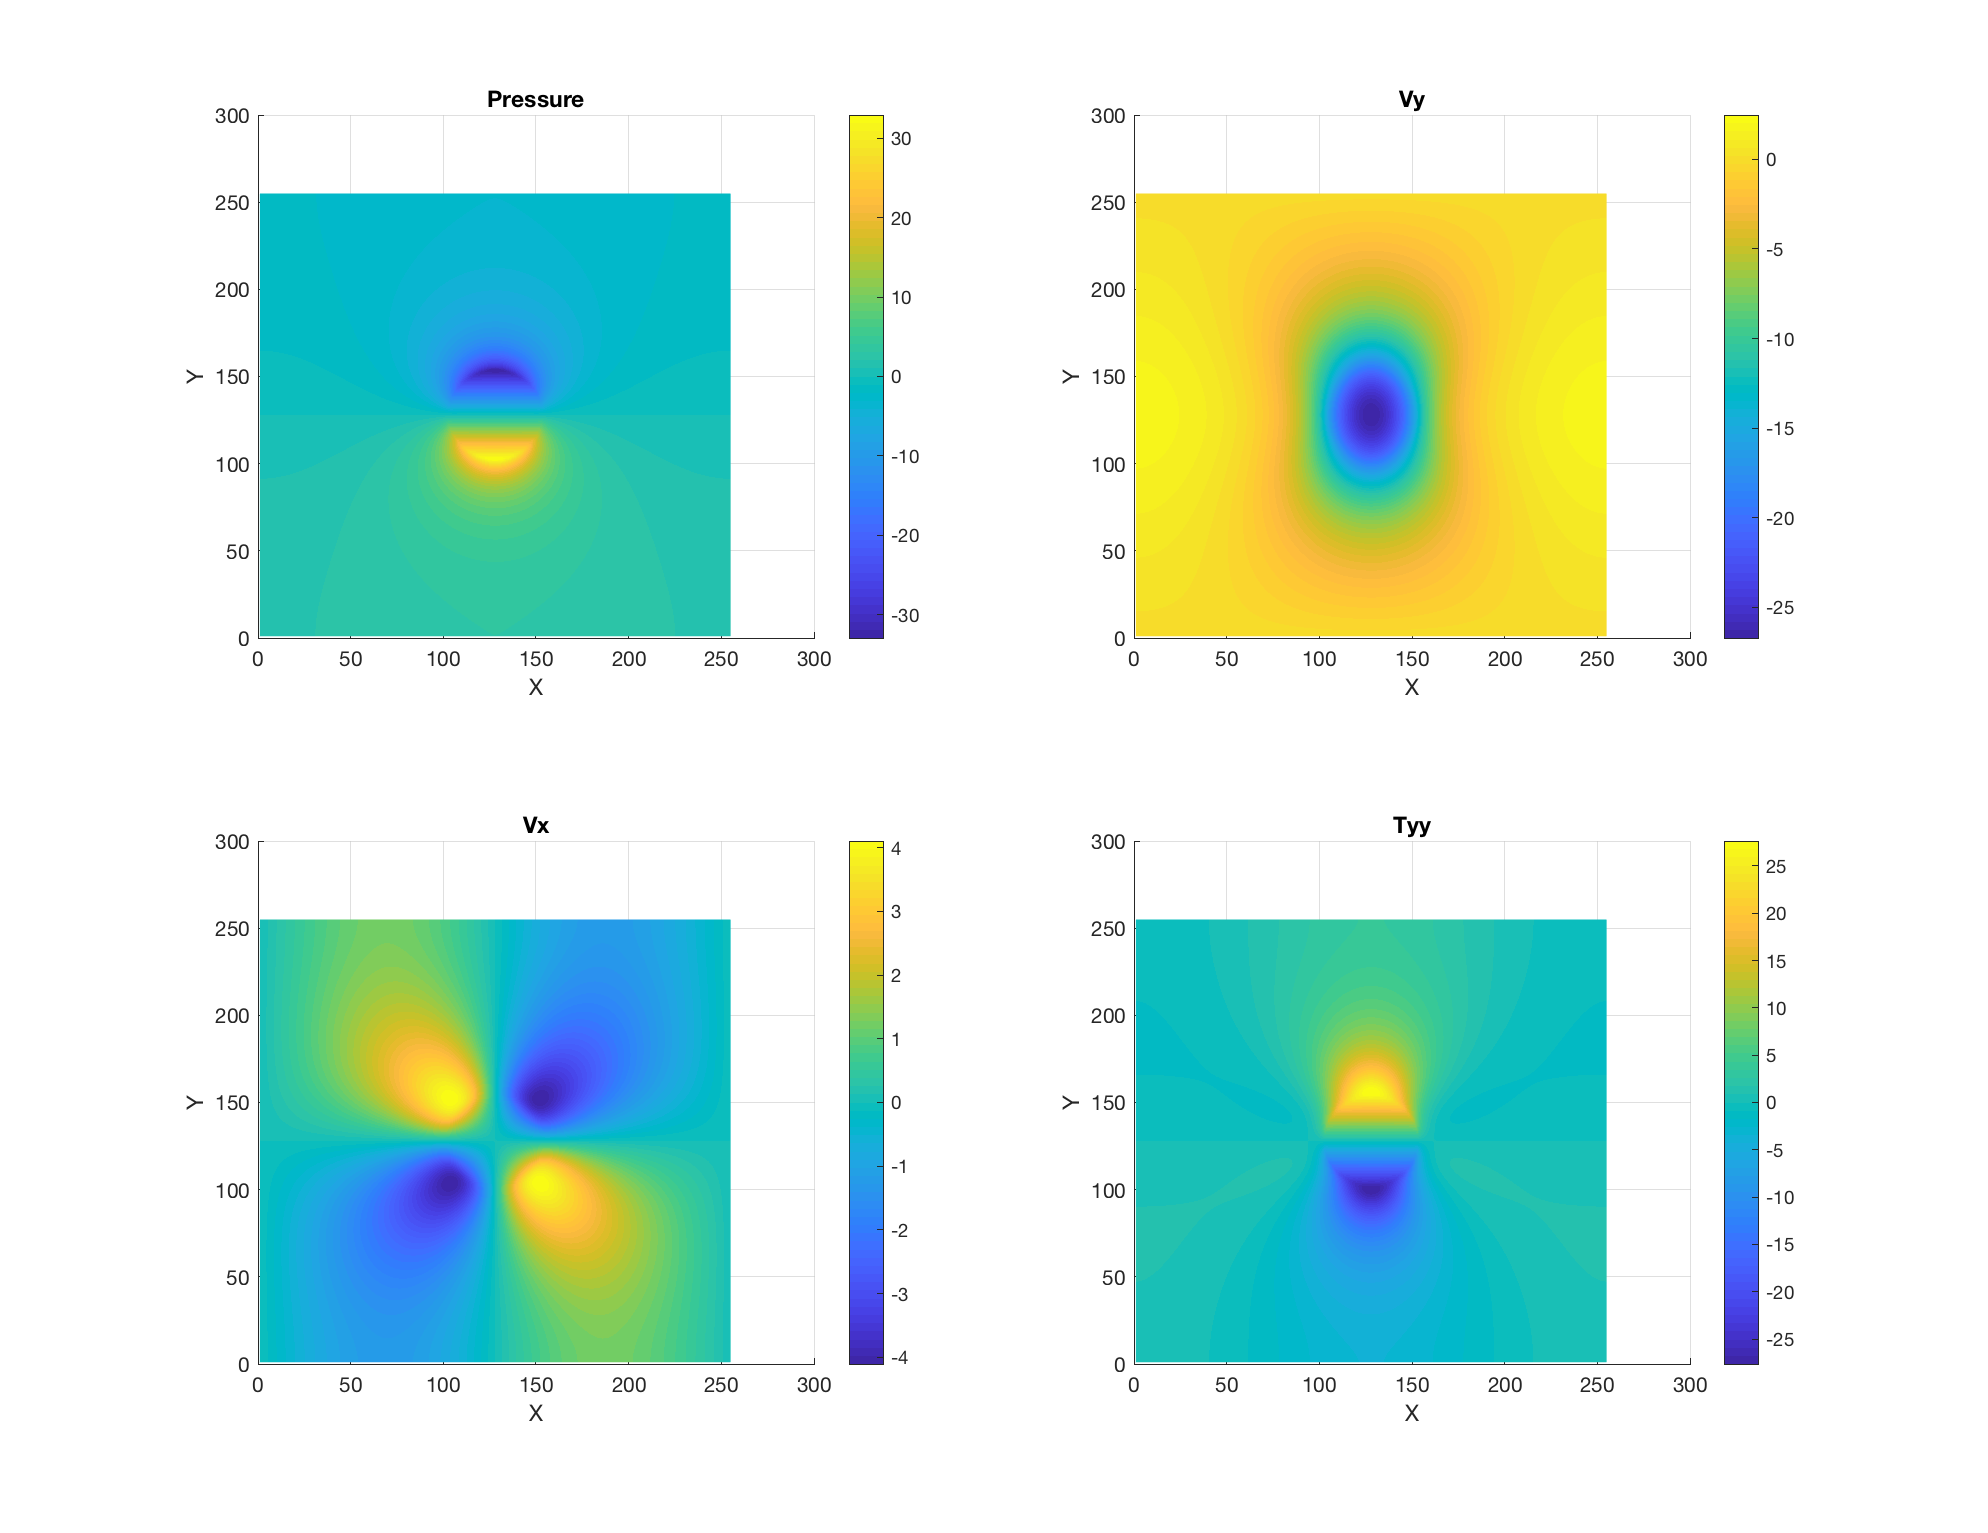
\includegraphics[width = .8\textwidth]{../3dvis/plots2d.png}
\end{center}
3D plot of final solution (255x255x255 run)
\begin{center}
	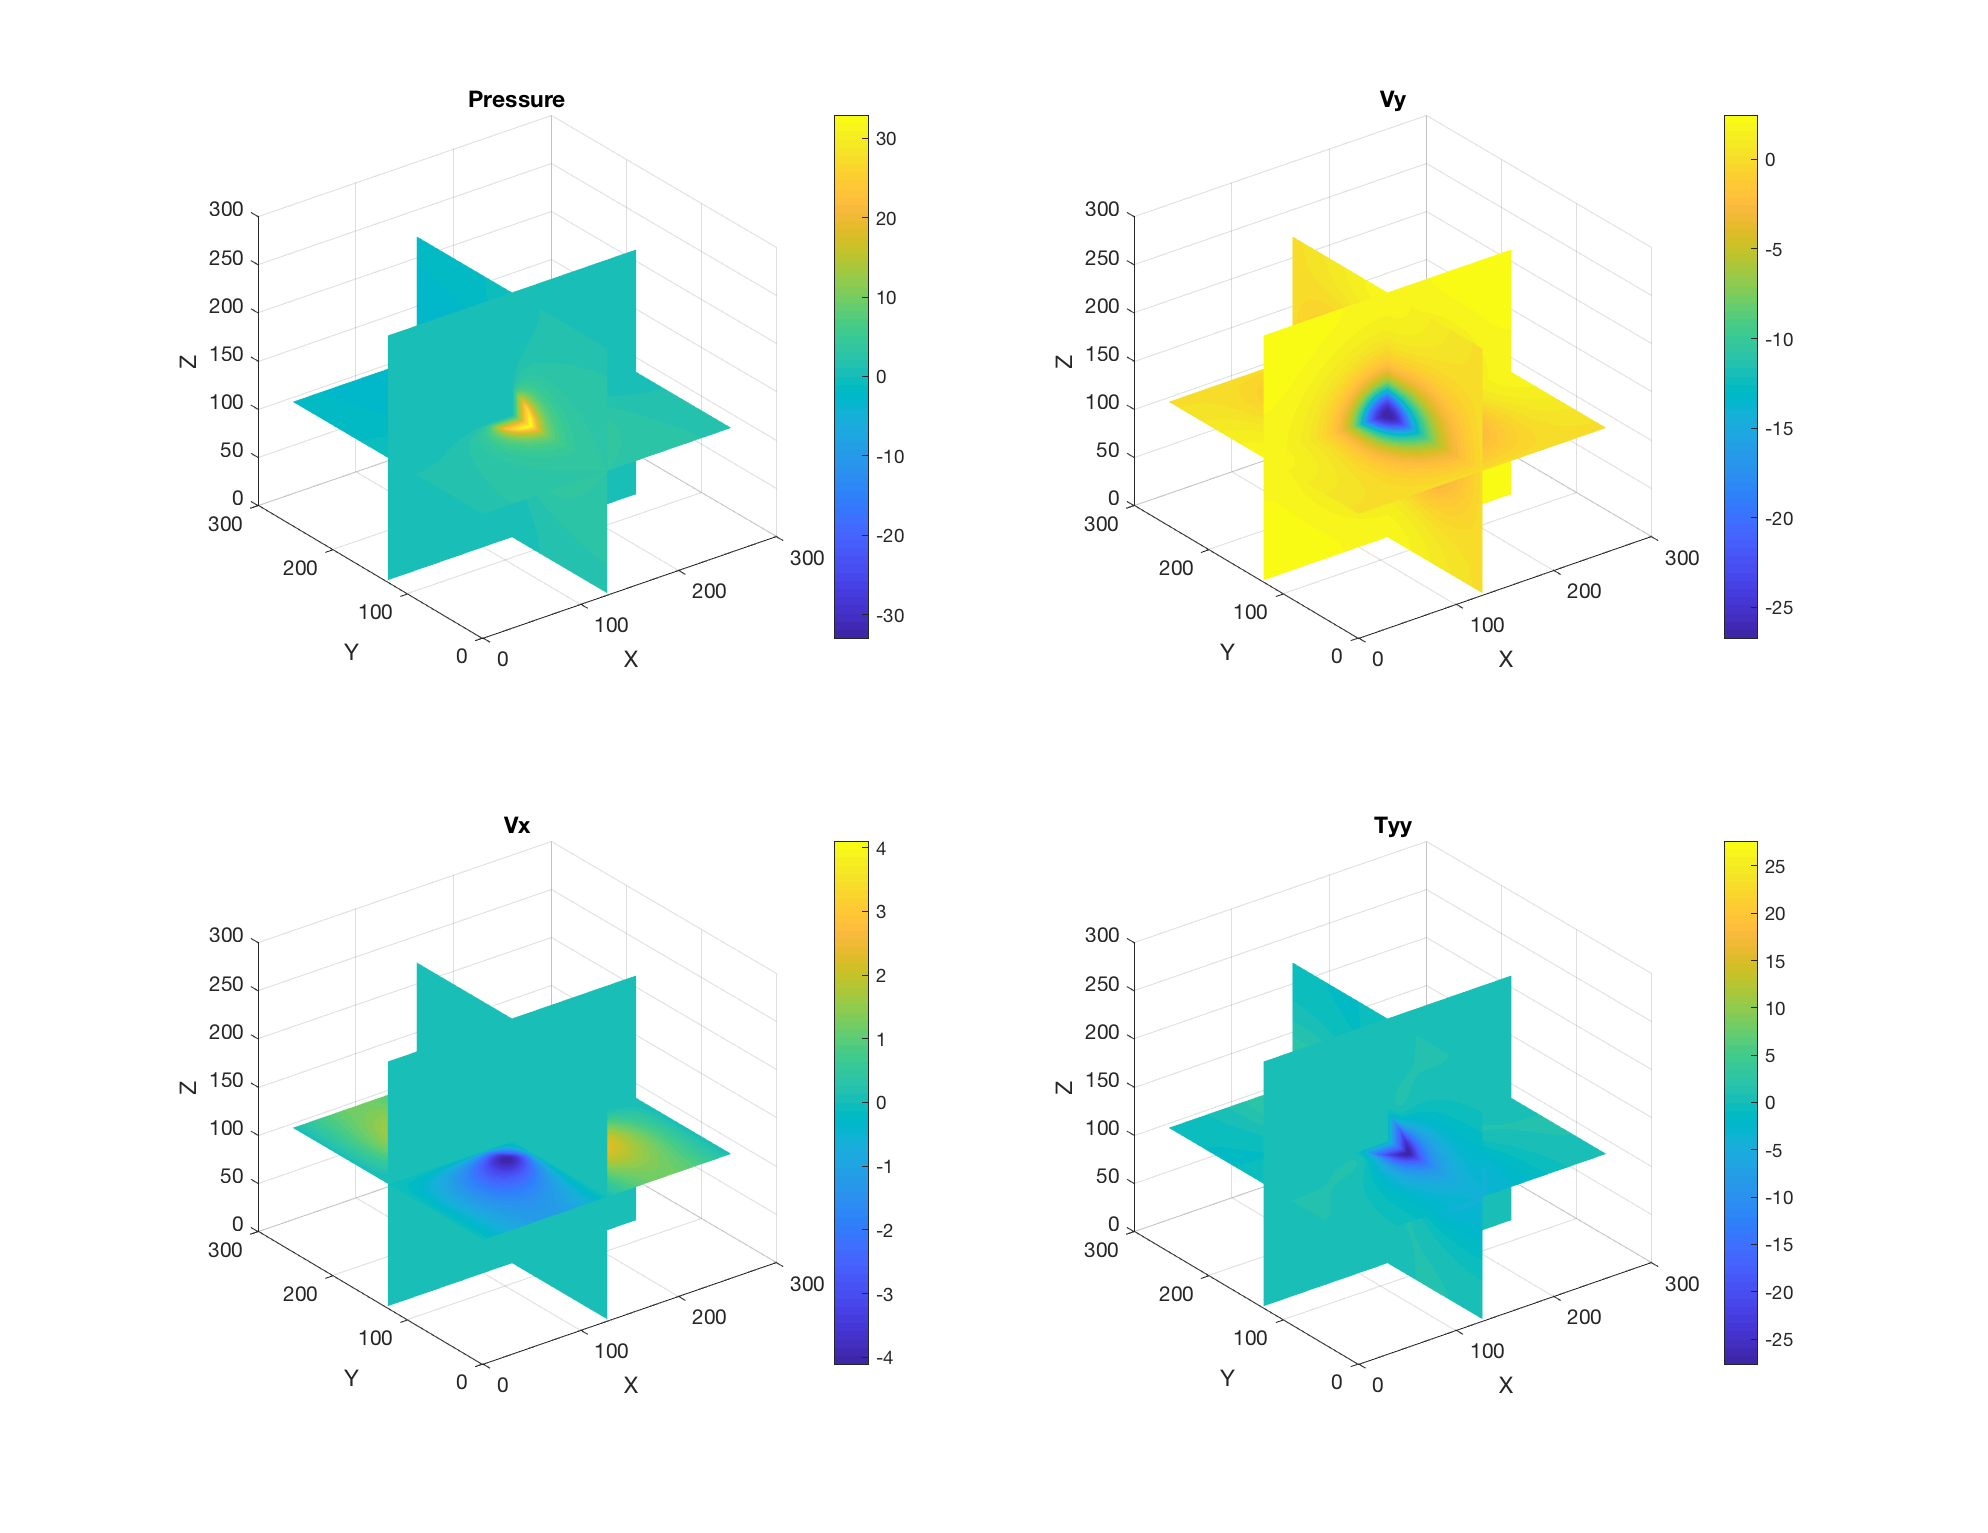
\includegraphics[width = .8\textwidth]{../3dvis/plots.png}
\end{center}

MTP Plot. We see nice saturation up to a peak value close to MTP\textsubscript{max} after at a size of around 100 per axis. This value is slightly over the max theoretical, which suggests that this value is likely slightly mis-calibrated, this is discussed more below.\\
\begin{center}
	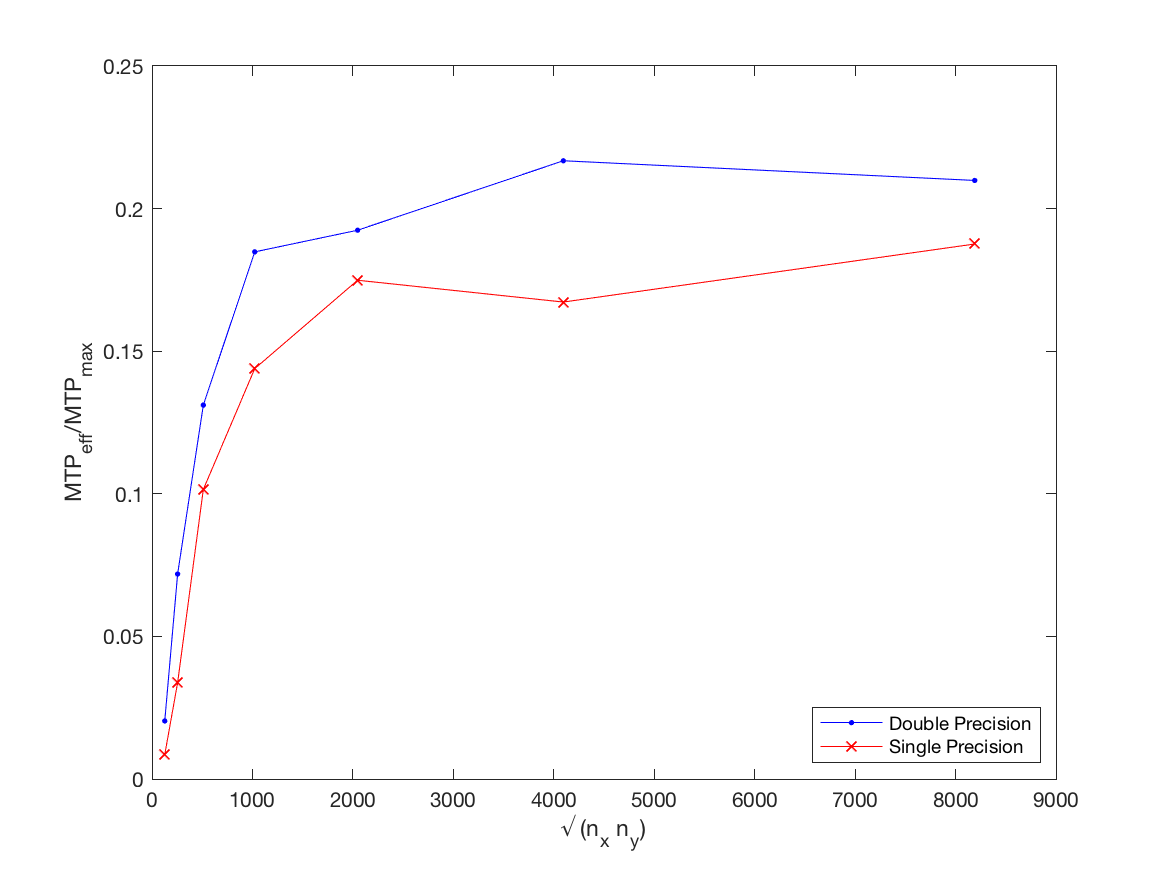
\includegraphics[width = .8\textwidth]{../3dvis/runTimes.png}
\end{center}
Convergence with resolution increase. We see nice conversion to the peak resolution run. We take the 255x255x255 run to be ground truth for this convergence test.\\
\begin{center}
	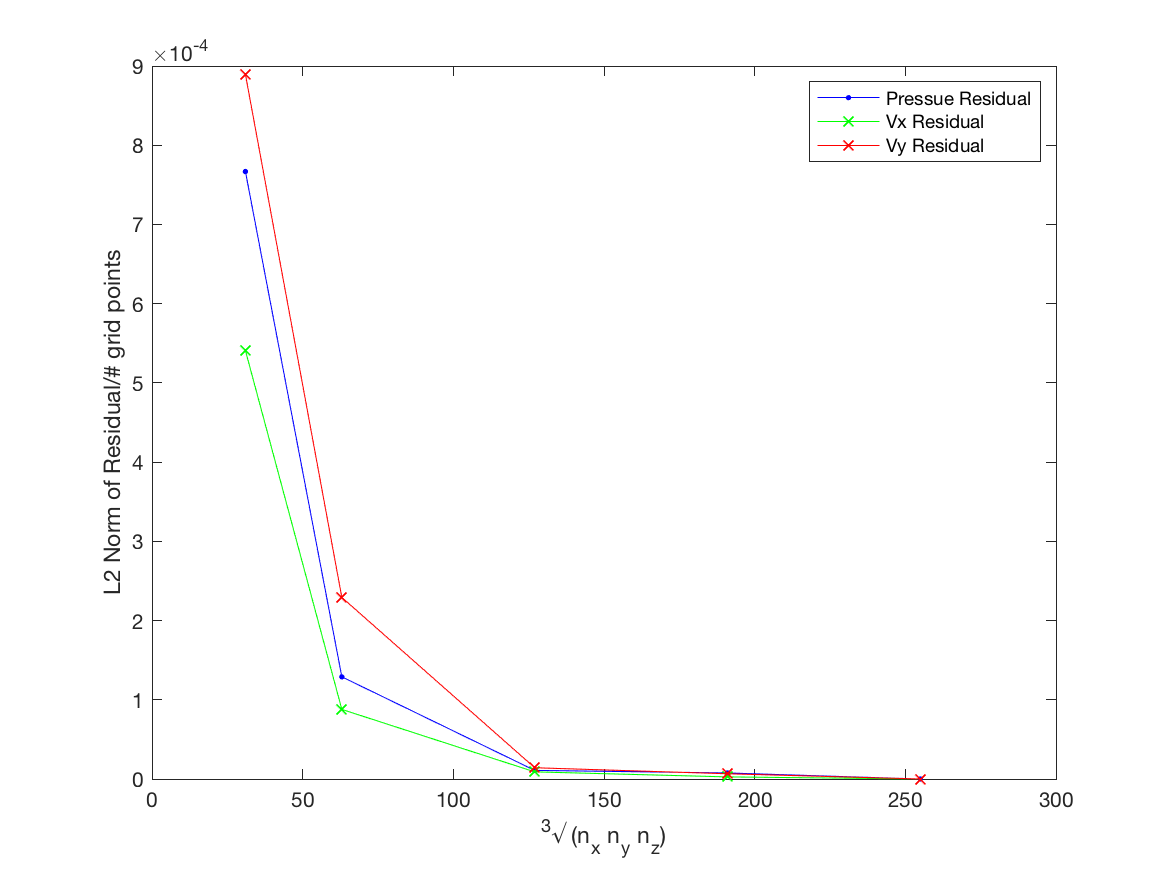
\includegraphics[width = .8\textwidth]{../3dvis/resids.png}
\end{center}
Convergence check in code, plot of iterations to converge. We see a nice linear trend in iterations needed to converge as grid size grows. This linear trend is confirmation that our accelerated pseudo-time convergence approach is working as desired.\\
\begin{center}
	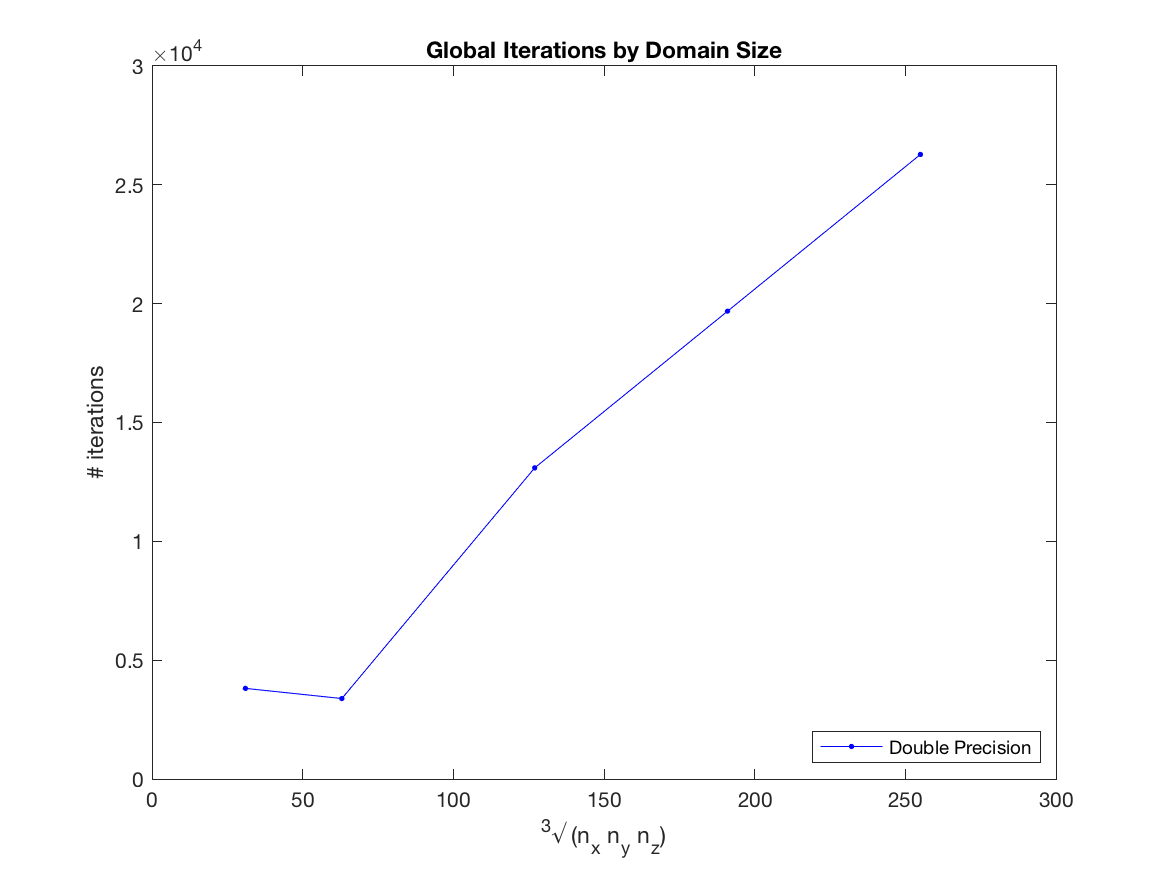
\includegraphics[width = .8\textwidth]{../3dvis/iterations.png}
\end{center}
% section results (end)
\section*{\myfont Discussion} % (fold)

% section discussion (end)
\section*{\myfont Conclusion} % (fold)

% section conculsion (end)
\end{document}
